% Created from docs/ambiguities/template.tex; questions remain optional later review.
\documentclass[a4paper,12pt]{article}
\usepackage[margin=19mm]{geometry}
\usepackage{amsmath,amssymb,graphicx,xcolor}
\usepackage{fontspec}
\usepackage{xepersian}
\settextfont{XB Roya}
\setlatintextfont{Latin Modern Roman}
\definecolor{ink}{HTML}{173D75}
\graphicspath{{images/}}
\setlength{\parindent}{0pt}
\setlength{\parskip}{5pt}
\linespread{1.12}
\newcommand{\qtitle}[2]{{\Large\bfseries\color{ink} پرسش \lr{#1}: #2}\par}
\newcommand{\answer}{\par\medskip\textbf{پاسخ یا صورت مورد تأیید و تاریخ:}\par\vspace{18mm}\hrule\medskip}
\begin{document}
{\LARGE\bfseries پرسش‌های ابهام جلسهٔ \lr{16}}\par
{\large جزوهٔ جبر پیشرفتهٔ دکتر خسروی}\par
شمارهٔ صفحه‌ها، شمارهٔ یک‌مبنای صفحه در فایل پی‌دی‌اف است، نه شمارهٔ دست‌نویس.
این پرسش‌ها برای بازبینی بعدی‌اند؛ خوانش‌های موقت در اسلایدها مشخص شده‌اند و
تکمیل گذر رونویسی به دریافت پاسخ وابسته نیست.
\medskip\hrule\medskip

\qtitle{L16-Q01}{نام نگاشت در اثبات یک‌به‌یکی}
\textbf{وضعیت:} باز؛ خوانش موقت ثبت شده است. تا \lr{2026-10-25} پاسخی دریافت نشده است.\par
\textbf{نشانی منبع:} نسخهٔ \lr{primary}، صفحهٔ \lr{5}، اثبات قرمزِ بالای صفحه،
بلافاصله پس از \(n\in\ker g=\operatorname{Im}f\).
\begin{LTR}\footnotesize
\texttt{sources/lectures/}\\
\texttt{16 Nakayama Lemma and Exact sequences .pdf}
\end{LTR}
\textbf{عبارت منبع:} پس از انتخاب \(m\in M\)، دست‌نویس می‌گوید \(g(m)=n\).
در نمودار، \(f:M\to N\) و \(g:N\to K\) هستند؛ سطر بعد از \(\beta f(m)\) استفاده می‌کند.
\begin{center}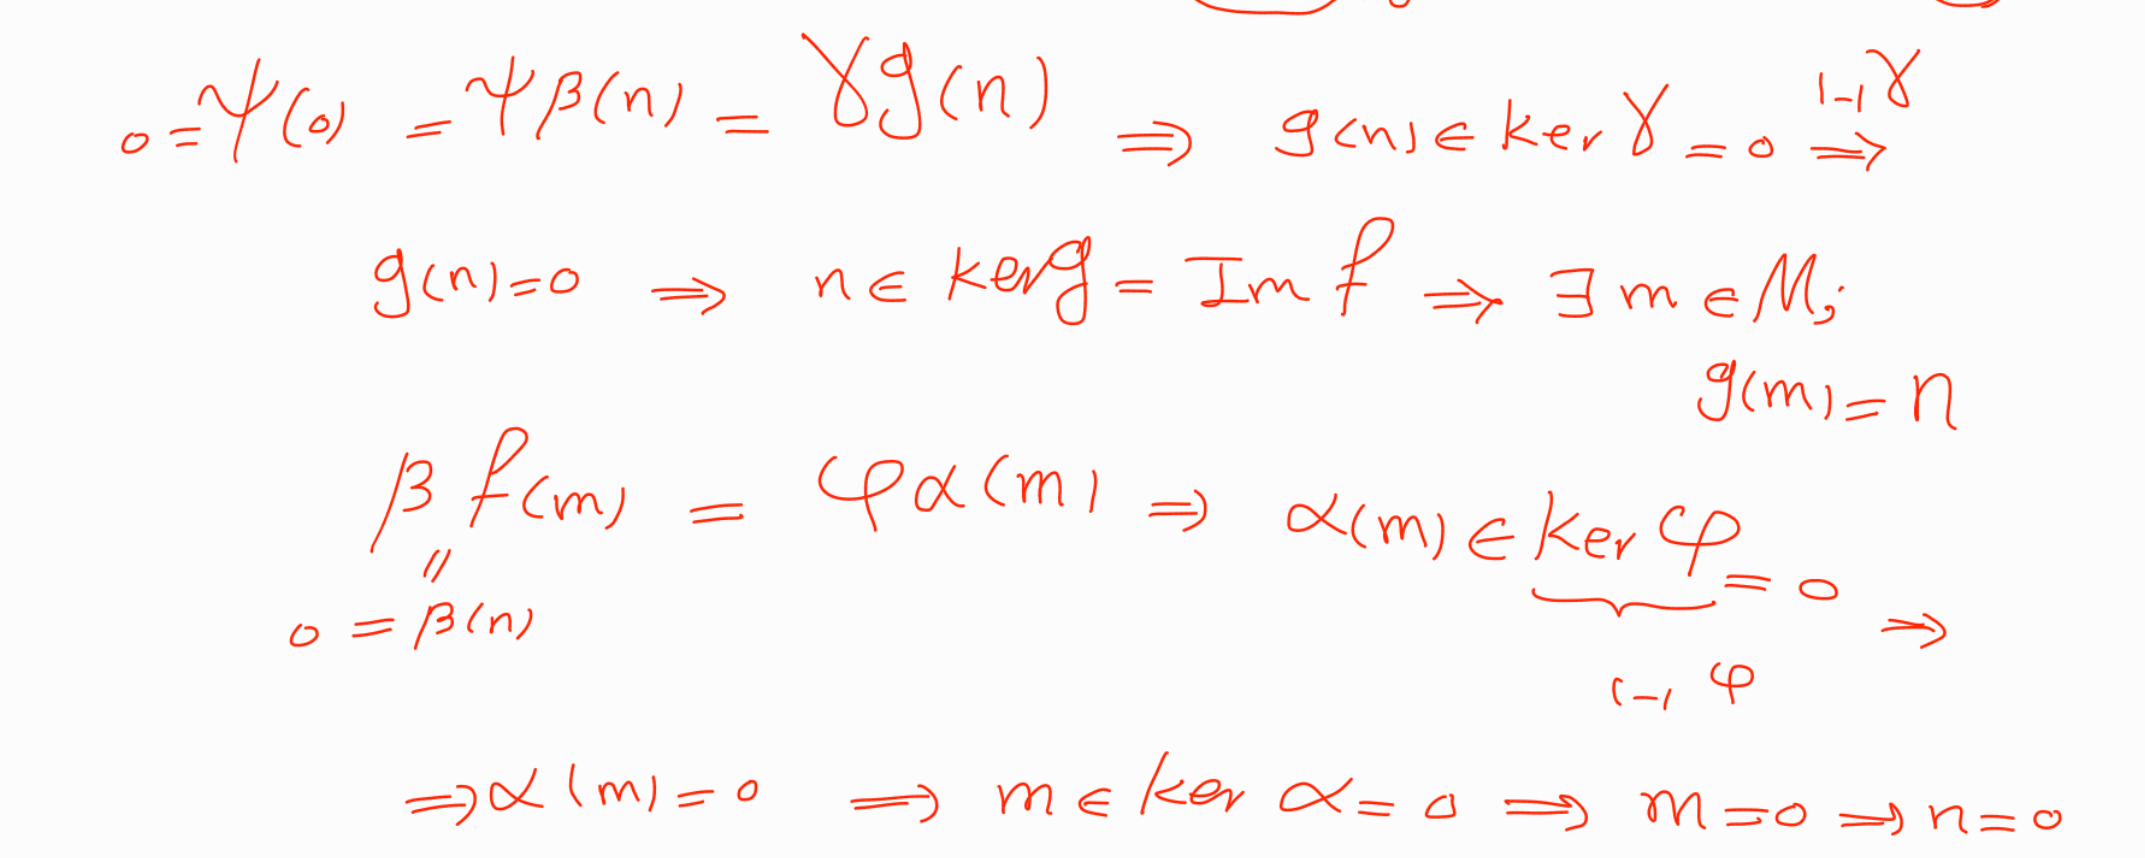
\includegraphics[width=\linewidth]{p05-missing-preimage.png}\end{center}
\textbf{خوانش‌ها و اثر تفاوت:}
خوانش لفظی \(g(m)=n\) با دامنه و هم‌دامنهٔ نگاشت‌های نمودار سازگار نیست.
خوانش پیشنهادی \(f(m)=n\) از \(n\in\operatorname{Im}f\) و سطر بعد پشتیبانی می‌گیرد
و گامِ انتخاب پیش‌تصویر را معتبر می‌کند.

\textbf{پرسش برای بازبینی بعدی:} آیا در این سطر، به جای \(g(m)=n\)،
رابطهٔ \(f(m)=n\) مورد نظر است؟

\textbf{تصمیم موقت:} در دو اسلاید اثبات یک‌به‌یکی، \(f(m)=n\) با برچسب خوانش موقت
به کار رفته است. ارجاع‌های بعدی به اثبات لم پنج‌تایی نیز این یادداشت را حفظ می‌کنند؛
اصلاح نماد، تأییدشده تلقی نشده است.
\answer

\newpage
\qtitle{L16-Q02}{تفاوت شاخص‌های \(t\) و \(k\) در جایگذاری}
\textbf{وضعیت:} باز؛ قرارداد شاخص‌ها موقت است. تا \lr{2026-10-25} پاسخی دریافت نشده است.\par
\textbf{نشانی منبع:} نسخهٔ \lr{primary}، صفحهٔ \lr{1}،
رابطهٔ \(m_1=\sum r_ix_i\) در میانهٔ صفحه و ضریب \(m_1\) در رابطهٔ «با جایگذاری» در نیمهٔ پایین.
\begin{LTR}\footnotesize
\texttt{sources/lectures/}\\
\texttt{16 Nakayama Lemma and Exact sequences .pdf}
\end{LTR}
\textbf{عبارت‌های منبع:} تعداد مولدها \(k\) است؛ نمایش \(m_1\) نیز \(t\) جمله دارد.\par
با این حال، ضریبِ جایگذاری‌شده با \(r_k\alpha_{k1}\) پایان می‌یابد:
\[
    m_1=r_1x_1+\cdots+r_tx_t,
    \qquad r'_1=r_1\alpha_{11}+\cdots+r_k\alpha_{k1}.
\]
\begin{center}

\includegraphics[width=\linewidth]{p01-initial-sum.png}\\[3pt]
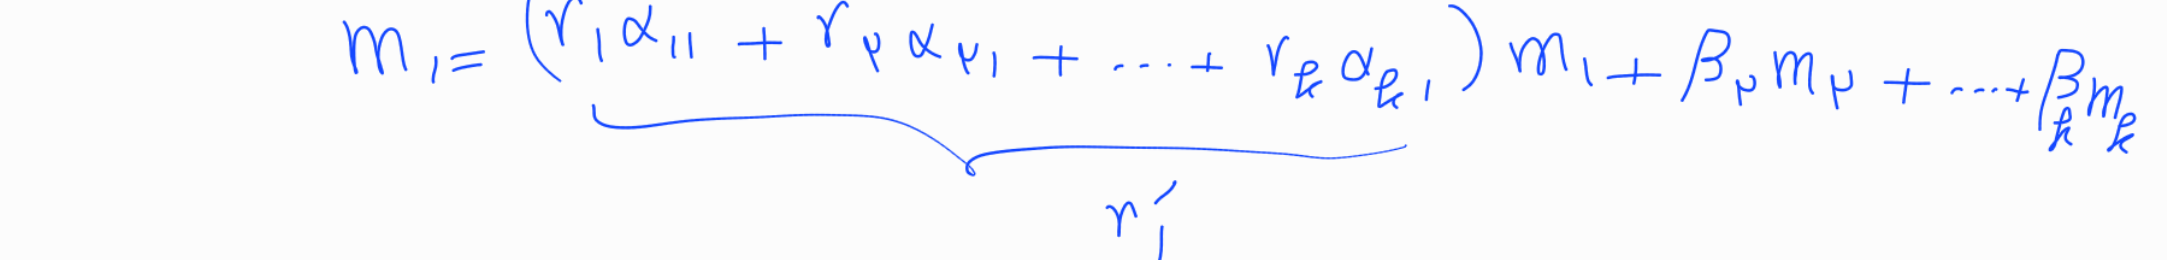
\includegraphics[width=\linewidth]{p01-substituted-sum.png}
\end{center}
\textbf{خوانش‌ها و اثر تفاوت:}
خوانش لفظی، دو شمارندهٔ مستقلِ تعداد مولدها و تعداد جمله‌ها را با هم جابه‌جا می‌کند؛
در منبع فرضی مانند \(t=k\) دیده نمی‌شود.
خوانش پیشنهادی این است که شاخصِ جمع بر جمله‌های نمایش اول حرکت کند:
\[
    x_i=\sum_{j=1}^{k}\alpha_{ij}m_j\quad(1\le i\le t),
    \qquad r'_1=\sum_{i=1}^{t}r_i\alpha_{i1}.
\]
این قرارداد با جایگذاری سازگار است؛ عضویت ضریب در \(J(R)\) نیز با دوطرفه بودن آن نتیجه می‌شود.

\textbf{پرسش برای بازبینی بعدی:} آیا کران ضریبِ جایگذاری باید \(t\) باشد،
یا در نمایش اولیه قرارداد دیگری برای شاخص‌ها مورد نظر بوده است؟

\textbf{تصمیم موقت:} در اسلاید جایگذاری، کران \(t\) با برچسب موقت استفاده شده است؛
پایان اثبات ناکایاما نیز به همین قرارداد ارجاع می‌دهد. متن لفظی و شاهد بالا برای بازبینی حفظ شده‌اند.
\answer
\end{document}
